%
% 02_kreis.tex -- Beweis des Satzes von Jordan für Kreise
%
% (c) 2026 Dominik Castelberg, Ostschweizer Fachhochschule
%
% !TEX root = ../../buch.tex
% !TEX encoding = UTF-8
%
\section{Der naive Ansatz: Form-spezifische Beweise
\label{jordan:section:kreis}}
\kopfrechts{Naive Ansätze für den Beweis}

Wie bereits erwähnt, ist der Satz von Jordan für spezielle Kurvenformen wie Kreise oder Ellipsen trivial zu beweisen.
So wäre der Beweis für eine Kreisform $\gamma(t) = (r \cos(2\pi t), r \sin(2\pi t))$ mit $t \in [0,1]$ und $r > 0$ einfach zu führen, da die Konstruktion der Kurve die Ebene zwangsläufig in ein inneres Gebiet (den Kreis) und ein äusseres Gebiet (die unendliche Fläche ausserhalb des Kreises) teilt.

\begin{proof}[Beweis des Satzes von Jordan für Kreise\label{jordan:beweis:jordan_kreis}]
    Sei $\gamma(t) = (r \cos(2\pi t), r \sin(2\pi t))$ eine einfache geschlossene Kurve in der Ebene $\mathbb{R}^2$. 
    Das innere Gebiet $I$ ist definiert als die Menge aller Punkte $(x,y)$, die die Ungleichung $x^2 + y^2 < r^2$ erfüllen. 
    Das äussere Gebiet $A$ ist definiert als die Menge aller Punkte $(x,y)$, die die Ungleichung $x^2 + y^2 > r^2$ erfüllen. 
    Die Kurve $\gamma$ selbst bildet den gemeinsamen Rand dieser beiden Gebiete, da sie die Gleichung $x^2 + y^2 = r^2$ erfüllt.    
    Daher hält der Satz von Jordan für Kreise.
\end{proof}

\begin{figure}
    \centering
    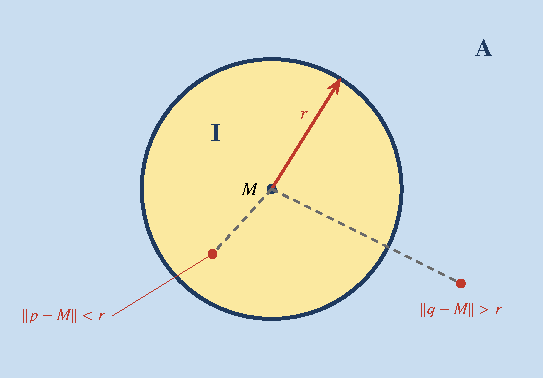
\includegraphics{papers/jordan/images/beweis_kreis.pdf}
    \caption{Aufteilung der Ebene $E$ durch eine Kreisform in ein inneres Gebiet $I$ und ein äusseres Gebiet $A$.}
\end{figure}

Doch dieser Beweis ist stark auf die spezielle Form der Kurve angewiesen und lässt sich nicht auf beliebige einfache geschlossene Kurven verallgemeinern. 
Da es potentiell unendlich viele verschiedene Formen von einfachen geschlossenen  Kurven gibt, ist es unmöglich, für jede Form einen eigenen Beweis zu führen. 
Dies macht den Ansatz form-spezifischer Beweise unpraktikabel und ineffizient.